\documentclass[11pt,aspectratio=169]{beamer}

% 直接复用现有主题配置。
% 通用宏包集中在此处；课程内容文件中通常不应再加载宏包。
\usepackage{iftex}
\ifPDFTeX
  \usepackage[T1]{fontenc}
  \usepackage[utf8]{inputenc}
  \usepackage{lmodern}
\else
  \usepackage{fontspec}
  \defaultfontfeatures{Ligatures=TeX}
\fi

\usepackage{amsmath,amssymb,mathtools}
\usepackage{booktabs}
\usepackage{graphicx}
\usepackage{tikz}
\usetikzlibrary{arrows.meta,positioning,shapes.geometric}
\usepackage[most]{tcolorbox}
\usepackage{listings}
\usepackage{xparse}
\usepackage{appendixnumberbeamer}
\usepackage[backend=biber,style=authoryear,maxcitenames=2]{biblatex}
% 修改整套课件配色时，只需要编辑本文件。
\definecolor{Primary}{HTML}{003B6F}
\definecolor{PrimaryLight}{HTML}{EAF2F8}
\definecolor{Accent}{HTML}{D97706}
\definecolor{AccentLight}{HTML}{FFF4E5}
\definecolor{Background}{HTML}{FFFFFF}
\definecolor{Text}{HTML}{20252B}
\definecolor{MutedText}{HTML}{66717E}
\definecolor{RuleColor}{HTML}{D7DEE5}
\definecolor{Success}{HTML}{237A57}
\definecolor{SuccessLight}{HTML}{EAF6F0}
\definecolor{CodeBackground}{HTML}{F5F7F9}
% 字体语义集中定义，避免在每一页手动设置字号与字重。
\ifPDFTeX
  \usefonttheme{professionalfonts}
\else
  \IfFontExistsTF{TeX Gyre Heros}{
    \setsansfont{TeX Gyre Heros}
  }{
    \setsansfont{Latin Modern Sans}
  }
  % TeX Gyre Cursor 随常见 TeX Live 安装提供，适合作为可移植的代码字体。
  \setmonofont{TeX Gyre Cursor}
\fi

\newcommand{\TitleFont}{\fontsize{25}{30}\selectfont\bfseries}
\newcommand{\SubtitleFont}{\large}
\newcommand{\FrameTitleFont}{\large\bfseries}
\newcommand{\BodyFont}{\normalsize}
\newcommand{\SmallFont}{\small}
\newcommand{\CodeFont}{\ttfamily\small}
% Beamer 外观：白底、蓝色主色、无导航按钮、极简页脚。
\mode<presentation>

\useinnertheme{rectangles}
\usefonttheme{professionalfonts}
\setbeamertemplate{navigation symbols}{}
\setbeamertemplate{headline}{}
\setbeamersize{text margin left=0.75cm,text margin right=0.75cm}

\setbeamercolor{normal text}{fg=Text,bg=Background}
\setbeamercolor{structure}{fg=Primary}
\setbeamercolor{alerted text}{fg=Accent}
\setbeamercolor{frametitle}{fg=Primary,bg=Background}
\setbeamercolor{title}{fg=Primary}
\setbeamercolor{subtitle}{fg=MutedText}
\setbeamercolor{author}{fg=Text}
\setbeamercolor{institute}{fg=MutedText}
\setbeamercolor{date}{fg=MutedText}
\setbeamercolor{itemize item}{fg=Primary}
\setbeamercolor{itemize subitem}{fg=Accent}
\setbeamercolor{section in toc}{fg=Text}
\setbeamercolor{section in toc shaded}{fg=MutedText}

\setbeamerfont{frametitle}{series=\bfseries,size=\large}
\setbeamerfont{title}{series=\bfseries,size=\LARGE}
\setbeamerfont{footline}{size=\scriptsize}

\setbeamertemplate{frametitle}{%
  \vspace{0.18cm}%
  \insertframetitle\par
  \vspace{0.10cm}%
  {\color{RuleColor}\rule{\textwidth}{0.5pt}}%
}

\setbeamertemplate{footline}{%
  \leavevmode
  \hbox{%
    \begin{beamercolorbox}[wd=.78\paperwidth,ht=2.8ex,dp=1.2ex,leftskip=.75cm]{normal text}%
      \color{MutedText}\insertshorttitle\enspace |\enspace\insertshortauthor
    \end{beamercolorbox}%
    \begin{beamercolorbox}[wd=.22\paperwidth,ht=2.8ex,dp=1.2ex,rightskip=.75cm plus1fil]{normal text}%
      \hfill\color{MutedText}\insertframenumber\,/\,\inserttotalframenumber
    \end{beamercolorbox}%
  }
}

\setbeamertemplate{title page}{%
  \vfill
  {\color{Primary}\rule{1.2cm}{3pt}\par}
  \vspace{0.55cm}
  {\TitleFont\color{Primary}\inserttitle\par}
  \vspace{0.18cm}
  {\SubtitleFont\color{MutedText}\insertsubtitle\par}
  \vspace{0.9cm}
  {\BodyFont\insertauthor\par}
  {\SmallFont\color{MutedText}\insertinstitute\par}
  \vspace{0.35cm}
  {\SmallFont\color{MutedText}\insertdate\par}
  \vfill
}

\setbeamertemplate{section page}{%
  \vfill
  {\color{MutedText}\large Chapter \insertsectionnumber\par}
  \vspace{0.25cm}
  {\color{Primary}\rule{1.2cm}{3pt}\par}
  \vspace{0.45cm}
  {\fontsize{27}{32}\selectfont\bfseries\color{Primary}\insertsectionhead\par}
  \vfill
}

\AtBeginSection[]{
  \begin{frame}[plain,noframenumbering]
    \sectionpage
  \end{frame}
}

\mode<all>
% 页面级语义环境。正文优先使用这些环境，而不是直接使用 frame。
\newenvironment{titleframe}
  {\begin{frame}[plain,noframenumbering]\titlepage}
  {\end{frame}}

\newenvironment{outlineframe}[1][Outline]
  {\begin{frame}{#1}\tableofcontents[currentsection,hideothersubsections]}
  {\end{frame}}

\newenvironment{theoryframe}[1]
  {\begin{frame}{#1}}
  {\end{frame}}

\newenvironment{exampleframe}[1]
  {\begin{frame}{#1}}
  {\end{frame}}

\newenvironment{figureframe}[1]
  {\begin{frame}{#1}\centering}
  {\end{frame}}

% fragile 页面必须通过 environment=codeframe 告知 Beamer 外层环境名。
\newenvironment{codeframe}[1]
  {\begin{frame}[fragile,environment=codeframe]{#1}}
  {\end{frame}}

\newenvironment{summaryframe}[1][Summary]
  {\begin{frame}{#1}}
  {\end{frame}}

\newcommand{\figurecaption}[1]{%
  \par\vspace{0.35cm}{\small\color{MutedText}#1\par}%
}
% 内容组件：信息框、强调命令、代码样式与常用数学命令。
\tcbset{
  coursebox/.style={
    enhanced,
    boxrule=0pt,
    leftrule=2.5pt,
    arc=1pt,
    outer arc=1pt,
    left=7pt,right=7pt,top=6pt,bottom=6pt,
    fonttitle=\bfseries,
    before skip=6pt,after skip=6pt
  }
}

\newtcolorbox{definitionbox}[1][Definition]{
  coursebox,title=#1,colback=PrimaryLight,colframe=Primary,coltitle=Primary
}
\newtcolorbox{theorembox}[1][Theorem]{
  coursebox,title=#1,colback=PrimaryLight,colframe=Primary,coltitle=Primary
}
\newtcolorbox{proofbox}[1][Proof idea]{
  coursebox,title=#1,colback=SuccessLight,colframe=Success,coltitle=Success
}
\newtcolorbox{remarkbox}[1][Remark]{
  coursebox,title=#1,colback=CodeBackground,colframe=MutedText,coltitle=Text
}
\newtcolorbox{warningbox}[1][Warning]{
  coursebox,title=#1,colback=AccentLight,colframe=Accent,coltitle=Accent
}
\newtcolorbox{importantbox}[1][Important]{
  coursebox,title=#1,colback=AccentLight,colframe=Accent,coltitle=Accent
}

\newcommand{\keyterm}[1]{\textcolor{Primary}{\textbf{#1}}}
\newcommand{\coursecheck}{\textcolor{Success}{\ensuremath{\checkmark}}}

\lstdefinestyle{coursecode}{
  basicstyle=\CodeFont,
  backgroundcolor=\color{CodeBackground},
  keywordstyle=\color{Primary}\bfseries,
  commentstyle=\color{Success},
  stringstyle=\color{Accent},
  numbers=left,
  numberstyle=\tiny\color{MutedText},
  numbersep=8pt,
  frame=single,
  rulecolor=\color{RuleColor},
  framesep=7pt,
  showstringspaces=false,
  breaklines=true,
  columns=fullflexible,
  keepspaces=true,
  tabsize=2
}
\lstset{style=coursecode}

\newcommand{\R}{\mathbb{R}}
\newcommand{\N}{\mathbb{N}}
\tcbset{coursebox/.append style={colbacktitle=Background}}

\addbibresource{../Causal_Inference_C/Beamer/Reference list/bibliography.bib}

% Automatic transition slide for each subsection:
% large section title above, subsection title below.
\newcommand{\sectionsubsectionframe}{%
  \begin{frame}[plain,noframenumbering]
    \vspace{0.9cm}
    {\fontsize{30}{36}\selectfont\bfseries\color{Text}%
      \insertsectionhead\par}

    \vspace{0.45cm}
    \noindent
    {\color{Accent}\rule{1.2cm}{1.3pt}}%
    {\color{RuleColor}\rule{\dimexpr\textwidth-1.2cm\relax}{0.6pt}}

    \vspace{0.45cm}
    {\fontsize{22}{27}\selectfont\bfseries\color{Text}%
      \insertsubsectionhead\par}
    \vfill
  \end{frame}%
}

\AtBeginSubsection[]{\sectionsubsectionframe}
% 课程信息：以后通常只需要修改这里和正文内容。
\title[Causal Inference]{Causal Inference}
\subtitle{Selection on Observables}
\author[Zhaoyi]{Zhaoyi}
%\institute[Your University]{Your University}
\date{\today}

\begin{document}

\begin{titleframe}


\end{titleframe}


\begin{outlineframe}

\end{outlineframe}

\section{What is the problem?}


\begin{frame}
We already know that "Randomized Experiment" doesn't always applied in certain context. Therefore, we should try other methods.\\
The core question is: Can we relax RCT assumptions and still learn causal effects?\\
We can start with designing the assumptions first:
\begin{itemize}
  \item Treatment assignment $D_i$ is no longer random.
  \item Unconfoundedness assumption: We observe pretreatment covariates $X_i$;and condition on $X_i$, treatment behaves as if random.
\end{itemize}

Given unconfoundedness, we will identify and estimate the average treatment effect and ATET.
\pause
\textbf{What others do we need?}
\pause
i.i.d.
%For simplicity
\end{frame}
\begin{frame}{An example: empirical motivation}
First, I would like to show an example the professor told me in class.

The example is from a paper and I will later present some section of this paper regarding this video's topic.
\end{frame}



\begin{frame}{Does Job Training Raise Earnings?}

\subsection*{Can government-sponsored job-training programs improve labor-market outcomes?}

\textbf{Setting: LaLonde (1986) and the National Supported Work (NSW):}
\begin{itemize}
    \item Sample: Individuals observed 1974–1978
    \begin{itemize}
        \item[$\blacksquare$] Treated $N_T = 185$ -- enrolled in NSW
        \item[$\blacksquare$] Control $N_C = 429$ -- non-participants drawn from CPS/PSID
    \end{itemize}
    \item Outcome of interest: Real earnings in 1978 (three years post-entry, $re78$)
\end{itemize}

\begin{center}
\begin{tabular}{lcc}
\hline
& \multicolumn{2}{c}{\textbf{Mean (SD)}} \\
\cline{2-3}
& Control & Treated \\
\hline
Re78 & 6984 (7294) & 6349 (7867) \\
N & 429 & 185 \\
\hline
\end{tabular}
\end{center}

\textbf{Raw comparison:} A naïve estimate suggests a negative effect--contradicting experimental evidence.

\end{frame}


\begin{frame}
\begin{itemize}
    \item We have information about demographics and pre-program earnings ($re74, re75$).
\end{itemize}

$\implies$ Treated and control units differ systematically; in particular:

$\implies$ Treated workers seemed to earn less than controls \emph{ex ante}, signaling selection bias.

\begin{center}
\begin{tabular}{lcc}
\hline
& \multicolumn{2}{c}{\textbf{Mean (SD)}} \\
\cline{2-3}
Variable & Control & Treated \\
\hline
education & 10.24 (2.86) & 10.35 (2.01) \\
hispanic & 0.14 (0.35) & 0.06 (0.24) \\
black & 0.20 (0.40) & 0.84 (0.36) \\
age & 28.03 (10.79) & 25.82 (7.16) \\
married & 0.51 (0.50) & 0.19 (0.39) \\
\hline
nodegree & 0.60 (0.49) & 0.71 (0.46) \\
re74 & 5619 (6788) & 2096 (4887) \\
re75 & 2466 (3292) & 1532 (3219) \\
Re78 & 6984 (7294) & 6349 (7867) \\
N & 429 & 185 \\
\hline
\end{tabular}
\end{center}

Can we recover causal effects from \emph{observational data} using statistical methods?

\end{frame}



\begin{frame}{What did the researcher do?}
We have information about demographics and pre-program earnings.\\
We will find:
\begin{itemize}
  \item Treated and control units differ systematically
  \item Treated workers seemed to earn less than controls before treatment, it shows \textbf{selection bias}.
\end{itemize}

And here is the question: Can we recover causal effects from observational data using statistical methods?


\end{frame}
















\section{Selection on Observables}


\subsection{Framework}



\begin{frame}{Settings}
The setup is as ususal, we assume SUTVA, consider the covariates, and binary treatment \\
What we need to pay attention to are two assumptions:
\begin{itemize}
  \item Conditional Independence, Unconfoundedness
  \item Overlap
\end{itemize}
And my goal is to know the causal effect, i.e., $\tau_{ATE}$ and $\tau_{ATET}$
\end{frame}


\begin{frame}{Why Do We Condition on Covariates?}

\begin{itemize}
    \item A natural first comparison in program evaluation is the difference in mean outcomes between treated units ($D_i = 1$) and control units ($D_i = 0$).
    \item Why the naive contrast is often not credible:
    \begin{itemize}
        \item[$\blacksquare$] Treated and control groups may differ in background covariates $X_i$, such as age, education, race, or pre-program earnings.
        \item[$\blacksquare$] These pre-existing differences can confound the outcome gap leading to selection bias.
    \end{itemize}
    \item In LaLonde (1986), program participants and non-participants differ in important observed characteristics.
    \item Selection on observables seeks to address this by conditioning on relevant covariates $X_i$.
    \item The key assumption is: given $X_i$, participation in the program $D_i$ is independent of potential outcomes $(Y_i(0), Y_i(1))$.
\end{itemize}

\end{frame}


\begin{frame}{Covariates and Outcomes}

\begin{definitionbox}[Definition: Predetermined Covariates]
A variable $X_i$ is predetermined with respect to treatment $D_i$ if its value is not affected by the treatment status of unit $i$.
\end{definitionbox}
\begin{itemize}
    \item Such covariates are often referred to as pretreatment covariates.
    \item This does not imply that $X_i$ and $D_i$ are independent.
    \item Predetermined variables may be time-invariant, such as sex or year of birth, or measured before treatment, such as pre-program earnings.
\end{itemize}
\end{frame}


\begin{frame}{Covariates and Outcomes}

\begin{definitionbox}[Definition: Outcomes]
An outcome is a variable whose value may be affected by the treatment. We describe this using potential outcomes $Y_i(1)$ and $Y_i(0)$.
\end{definitionbox}
\begin{itemize}
    \item In general, we should not condition on variables that may themselves be affected by the treatment.
    \item Conditioning on post-treatment variables can introduce bias.
\end{itemize}

\end{frame}



\section{Identification}
\subsection{Assumptions}

\begin{frame}


\end{frame}


\begin{frame}{Assumption: Conditional Independence}

\begin{definitionbox}[Assumption: Conditional Independence]
Potential outcomes $(Y_i(0), Y_i(1))$ and treatment assignment $D_i$ are independent conditional on $X_i$:
$$(Y_i(0), Y_i(1)) \perp\!\!\!\perp D_i \mid X_i.$$
\end{definitionbox}
The conditional independence assumption is also known as unconfoundedness, selection on observables, or the missing at random assumption.
\end{frame}

\begin{frame}[Conditional Independence and Exogeneity Assumptions]

To see the connection with standard exogeneity assumptions, assume a constant treatment effect and a linear model for the untreated potential outcome:
$$Y_i(0) = \alpha + X_i^\top \beta + \varepsilon_i \quad \text{and} \quad Y_i(1) = Y_i(0) + \tau.$$

Then the observed outcome can be written as
$$Y_i = \alpha + \tau D_i + X_i^\top \beta + \varepsilon_i.$$

Under this setup, unconfoundedness implies that, conditional on $X_i$, treatment assignment is unrelated to the unobserved component $\varepsilon_i$.

In a regression framework, the key requirement is often the conditional mean restriction
$$\mathbb{E}[\varepsilon_i \mid D_i, X_i] = \mathbb{E}[\varepsilon_i \mid X_i],$$
which captures the idea that $D_i$ is exogenous once we condition on $X_i$.
\end{frame}











\subsection{Failure of Identifying Assumption}

\begin{frame}{Conditional Independence Assumption (CIA)}
\begin{definitionbox}[CIA]
Potential outcomes $(Y_i(0),Y_i(1))$ and treatment assignment $D_i$ are independent conditional on $X_i$:
$$(Y_i(0),Y_i(1))\perp D_i \vert X_i$$
\end{definitionbox}
\end{frame}

\begin{frame}{Conditional Mean Independence}

For many of the result in this chapter, it is indeed sufficient to impose a weaker assumption:

\begin{definitionbox}[Conditional Mean Independence]

Conditional on $X_i$, treatment assignment does not change the conditional means of the potential outcomes:
$$E[Y_i(0)\vert X_i,D_i]=E[Y_i(0)\vert X_i] \quad E[Y_i(1)\vert X_i,D_i]=E[Y_i(1)\vert X_i]$$

\end{definitionbox}
\end{frame}




\begin{frame}{Conditional Independence fails...}
\begin{itemize}
  \item Unconfoundedness is not directly testable because it is an assumption about unobserved potential outcomes.
  \item In any empirical setting, we need to assess whether the condition is plausible.
  \item Even though unconfoundedness is not testable, researchers often conduct \textbf{credibility checks}.
  \item What if key confounders are unobserved?
  \begin{itemize}
    \item If conditional independence is implausible, stronger research designs may be needed that we discuss the upcoming lectures.
    \item Without such strategies, one may only be able to identify bounds on treatment effects.
  \end{itemize}
\end{itemize}

\end{frame}


\begin{frame}
\end{frame}


\begin{frame}
\end{frame}





\begin{frame}{When Overlap fails: Trimming?}
\begin{itemize}
  \item Overlap problems can be diagnosed empirically. How should we estimate it?
  \item Regarding the propensity score, we need to examine the overlap problems:
  \begin{itemize}
    \item Inspect the estimated distribution of the propensity score.
    \item Look for regions where the estimated propensity score is close to 0 or 1
  \end{itemize}
  \item Trim the sample:
  \begin{itemize}
    \item Restrict the sample to the resion of common support, for example $\hat{e}(X_i)\in [0.05,0.95]$
    \item Report the treatment effect for the resulting subpopulation.
  \end{itemize}
  Therefore, trimming may improve credibility, but it changes the estimand.
\end{itemize}

\end{frame}


\subsection{Estimation and Inference}
\begin{frame}{From Identification to Estimation}



\end{frame}
\begin{frame}{Notation: Discrete Covariates}

\begin{itemize}
    \item Suppose $X_i$ is discrete and takes values in $\{x_1, \dots, x_k\}$.
    \item As in stratified experiments, partition the sample into covariate cells:
    \begin{center}
    \begin{tabular}{c|ccc}
    & $X_i = x_1$ & $\cdots$ & $X_i = x_k$ \\
    \hline
    $D_i = 0$ & $n_{0,x_1}$ & $\cdots$ & $n_{0,x_k}$ \\
    $D_i = 1$ & $n_{1,x_1}$ & $\cdots$ & $n_{1,x_k}$ \\
    \hline
    Total & $n_{x_1}$ & $\cdots$ & $n_{x_k}$
    \end{tabular}
    \end{center}
    \item For each cell $x$, let
    $$n_{d,x} = \#\{i : D_i = d, X_i = x\}, \quad n_x = n_{0,x} + n_{1,x}.$$
    \item Let $n_1$ and $n_0$ denote the total numbers of treated and untreated units.
    \item Finally, define the population cell shares
    $$\pi(x_j) = \Pr(X_i = x_j), \quad \pi(x_j \mid D_i = 1) = \Pr(X_i = x_j \mid D_i = 1).$$
\end{itemize}

\end{frame}


\begin{frame}{Estimators with Discrete Covariates}

\begin{definitionbox}{Estimation of the CATE}
The CATE is
$$\tau_{\text{CATE}}(x) = \mathbb{E}[Y_i(1) - Y_i(0) \mid X_i = x].$$
A natural estimator is the difference in average outcomes within the same covariate cell:
$$\widehat{\tau}_{\text{CATE}}(x) = \frac{1}{n_{1,x}} \sum_{i:D_i=1, X_i=x} Y_i - \frac{1}{n_{0,x}} \sum_{i:D_i=0, X_i=x} Y_i.$$
\end{definitionbox}
\end{frame}

\begin{frame}{Estimator for ATE with Discrete Covariates}

\begin{definitionbox}{Estimation of the ATE}
The ATE averages the CATE over the distribution of $X_i$:
$$\tau_{\text{ATE}} = \sum_{j=1}^k \pi(x_j) \tau_{\text{CATE}}(x_j), \quad \pi(x_j) = \Pr(X_i = x_j).$$
A natural estimator is
$$\widehat{\tau}_{\text{ATE}} = \sum_{j=1}^k \frac{n_{x_j}}{n} \widehat{\tau}_{\text{CATE}}(x_j).$$
\end{definitionbox}
This estimator requires that each relevant covariate cell contains both treated and control units.

\end{frame}

\begin{frame}{Asymptotic Normality with Discrete Covariates}

\begin{theorembox}{Theorem}
Suppose that unconfoundedness, weak overlap, and our regularity assumptions hold. It then follows that
$$\sqrt{n}(\widehat{\tau}_{\text{ATE}} - \tau_{\text{ATE}}) \xrightarrow{d} \mathcal{N}(0, V_{\text{ATE}}),$$
where
$$V_{\text{ATE}} = \mathbb{E}\left[\frac{\sigma_1^2(X_i)}{e(X_i)}\right] + \mathbb{E}\left[\frac{\sigma_0^2(X_i)}{1 - e(X_i)}\right] + \mathbb{E}\left[\{\tau_{\text{CATE}}(X_i) - \tau_{\text{ATE}}\}^2\right],$$
where $\sigma_d^2(X_i) = \mathbb{E}[(Y_i(d) - \mu_d(X_i))^2 \mid X_i]$.
\end{theorembox}
I will show the method of this proof, not formal but intuitive.
\end{frame}

\begin{frame}
For the further discussion to the Variance, I will also show it in another screen.

\end{frame}

\begin{frame}{Subclassification and the "Curse of Dimensionality"}


\end{frame}
\begin{frame}{Subclassification and the ``Curse of Dimensionality''}

\begin{itemize}
    \item Subclassification becomes unfeasible with many covariates.
    \item Assume we have $k$ covariates and divide each of them into 3 coarse categories (e.g., age: ``young'', ``middle age'' or ``old'', and income: ``low'', ``medium'' or ``high'').
    \item The number of subclassification cells is $3^k$. For $k = 10$, we obtain $3^{10} = 59,049$.
    \item Many cells may contain only treated or untreated observations, so we cannot use subclassification.
    \item Finer categories make the problem even more severe: with 5 categories per covariate and $k = 10$, we obtain $5^{10} = 9,765,625$ cells.
\end{itemize}
\end{frame}

\begin{frame}{Why Continuous Covariates are Hard}
I will introduce different approaches:
\begin{itemize}
  \item Regression Adjustment: Controlling for $X_i$ in a regression framework.
  \item Matching: Pairing units with similar $X_i$
  \item Propensity Score Weighting: Reweighting observations based on their probability of treatment.
  \item Combining Regression and Propensity Score Weighting: A hybrid approach.
\end{itemize}
\end{frame}


\section{Estimation Method for Continuous Covariates}
\begin{frame}
In this part I will introduce several matching methods.

\end{frame}

\subsection{Regression Adjustment}

\begin{frame}{Estimation: Regression Adjustment}

\begin{itemize}
    \item We now discuss how to estimate the ATE using regression adjustment.
    \item Remember that
    $$\tau_{\text{ATE}} = \mathbb{E}_X[\mathbb{E}(Y_i \mid X_i, D_i = 1)] - \mathbb{E}_X[\mathbb{E}(Y_i \mid X_i, D_i = 0)] \equiv \mathbb{E}_X[m(1, X_i) - m(0, X_i)].$$
    \item $m(d, X_i)$ is unknown and needs to be estimated.
    \begin{enumerate}
        \item[(0)] Select a parametric model for $m_\beta(d, X_i)$ (usually OLS, or logit or probit for binary outcomes).
        \item[(1)] Estimate $\widehat{\beta}$.
        \item[(2)] Use estimated $m_{\widehat{\beta}}(d, X_i)$ to compute regression adjusted estimates.
        \item[(3)] Average these estimates over the empirical distribution of $X_i$:
        $$\widehat{\tau}_{\text{ATE}} = \frac{1}{n} \sum_{i=1}^n \left[m_{\widehat{\beta}}(1, X_i) - m_{\widehat{\beta}}(0, X_i)\right].$$
    \end{enumerate}
\end{itemize}

\end{frame}


\begin{frame}{Consistency of Regression Adjustments}

\begin{theorembox}{Theorem: Consistency of Regression Adjustments}
Suppose that unconfoundedness and overlap hold and that all necessary moments exist. In addition, assume that:
\begin{enumerate}
    \item the outcome regression is correctly specified, i.e.
    $$\mathbb{E}[Y_i \mid X_i = x, D_i = d] = m_{\beta_0}(d, x)$$
    for some $\beta_0$ and $d \in \{0, 1\}$;
    \item $\widehat{\beta} \xrightarrow{p} \beta_0$;
    \item $m_\beta(d, x)$ is L-Lipschitz continuous in $\beta$ uniformly in $x$.
\end{enumerate}

Then the regression adjustment estimator is consistent for the ATE.
\end{theorembox}
\end{frame}


\begin{frame}{Regression Adjustment}

\begin{itemize}
    \item Under additional assumptions, one can show that the regression adjustment estimator is $\sqrt{n}$-asymptotically normal.
    \item However, both consistency and asymptotic normality rely on strong functional-form assumptions.
    \item We therefore also consider more flexible approaches below.
\end{itemize}

\end{frame}


\begin{frame}


\end{frame}









\subsection{Matching}

\begin{frame}{$M$ Nearest Neighbor Matching}

\begin{itemize}
    \item With discrete covariates, we can compare treated and untreated units with the same value of $X_i$.
    \item With continuous covariates, exact matches are typically unavailable.
    \item Matching therefore compares units with similar observed covariates.
    \item In $M$ nearest neighbor matching, each unit is matched to the $M$ closest units from the opposite treatment group.
\end{itemize}

\end{frame}


\begin{frame}{Matching: Intuition}
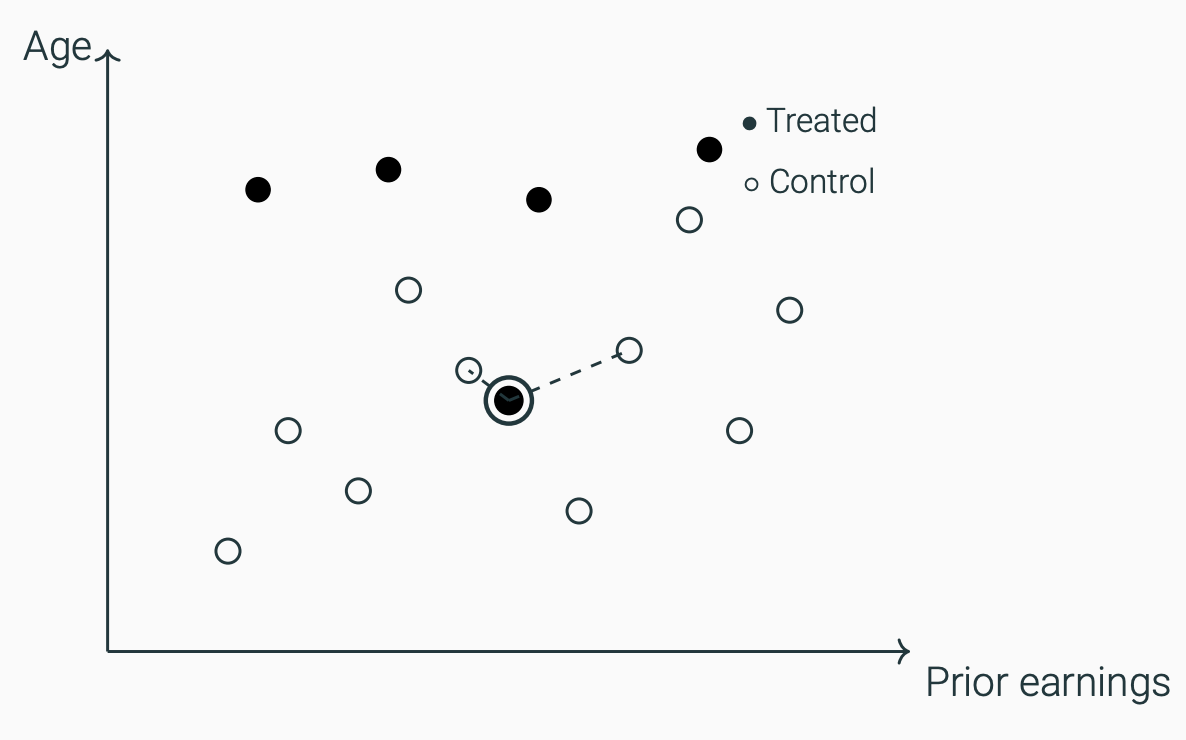
\includegraphics[width=0.5\textwidth]{Courses/image_7.png}
\begin{itemize}
    \item Matching imputes missing potential outcomes using similar units from the other treatment group.
    \item Similarity is measured by a distance metric $d(X_i, X_j)$.
    \item Good matches become harder to find as the dimension of $X_i$ increases.
\end{itemize}

\end{frame}
\begin{frame}{Estimation: $M$ Nearest Neighbor Matching}

\begin{enumerate}
    \item For each unit $i$, let $J_M(i)$ be the set of its $M$ nearest neighbors among units with $D_j = 1 - D_i$.
    \item Impute the missing potential outcomes:
    $$\widehat{Y}_i(0) = \begin{cases} \frac{1}{M} \sum_{j \in J_M(i)} Y_j, & \text{if } D_i = 1, \\ Y_i, & \text{if } D_i = 0, \end{cases} \qquad \widehat{Y}_i(1) = \begin{cases} Y_i, & \text{if } D_i = 1, \\ \frac{1}{M} \sum_{j \in J_M(i)} Y_j, & \text{if } D_i = 0. \end{cases}$$
    \item Average the imputed treatment effects:
    $$\widehat{\tau}_{\text{ATE}} = \frac{1}{n} \sum_{i=1}^n \left[\widehat{Y}_i(1) - \widehat{Y}_i(0)\right] \qquad \widehat{\tau}_{\text{ATET}} = \frac{1}{n_1} \sum_{i:D_i=1} \left[\widehat{Y}_i(1) - \widehat{Y}_i(0)\right],$$
    where $n_1 = \sum_{i=1}^n D_i$.
\end{enumerate}

\end{frame}

\begin{frame}{Mahalanobis Distance}

\begin{itemize}
    \item Mahalanobis distance rescales the covariates using their variance-covariance matrix.
    \item In the matching context, it is commonly defined as
    $$d(X_i, X_j) = \sqrt{(X_i - X_j)' \widehat{W}^{-1} (X_i - X_j)},$$
    where
    $$\widehat{W} = \frac{1}{n} \sum_{i=1}^n (X_i - \overline{X}_{D_i})(X_i - \overline{X}_{D_i})' \quad \text{and} \quad \overline{X}_d = \frac{1}{n_d} \sum_{i:D_i=d} X_i $$
    \item This metric accounts for differences in scale and correlation among the components of $X_i$.
\end{itemize}

\end{frame}


\begin{frame}{Basic Intuition}


\end{frame}


\begin{frame}{Discussion: $M$ Nearest Neighbor Matching}

Pros:
\begin{itemize}
    \item Matching is intuitive and avoids specifying a full outcome regression model.
    \item Balance and matching quality can be checked directly.
    \item The method works well when good matches are available.
\end{itemize}

Cons:
\begin{itemize}
    \item The researcher must choose $M$ and a distance metric.
    \item Good matches are difficult to find in high dimensions.
    \item Without bias correction, matching bias can invalidate standard $\sqrt{n}$ inference.
\end{itemize}

\end{frame}



\subsection{Propensity Score}

\begin{frame}{Why introduce the Propensity Score?}
\begin{itemize}
  \item Identification by conditioning on $X_i$ is conceptually simple.
  \item But when $X_i$ is high-dimensional, exact comparisons are often infeasible.
  \item The propensity score summarizes the covariates into the scalar while preserving the relevant comparability condition.
\end{itemize}
\end{frame}

\begin{frame}{Dimension Reduction}

\begin{itemize}
    \item Suppose there exists a function $b(X_i) \in \mathbb{R}^{k'}$ with $k' < k$ such that
    $$Y_i(0), Y_i(1) \perp\!\!\!\perp D_i \mid b(X_i) $$
    \item Then, one can reduce the dimension by replacing $X_i$ with $b(X_i)$.
    \item Interestingly, the propensity score $e(X_i) = P(D = 1 \mid X_i)$ satisfies this property:
    $$Y_i(0), Y_i(1) \perp\!\!\!\perp D_i \mid e(X_i) $$
\end{itemize}
\end{frame}
\begin{frame}{Definition: Balancing Score}
\begin{definitionbox}[Balancing Score]

A balancing score is a function $b(X_i)$ such that
$$D_i \perp\!\!\!\perp X_i \mid b(X_i) $$
\end{definitionbox}
\begin{theorembox}[Lemma: Balancing Property of the Propensity Score]
The propensity score $e(X_i)$ is a balancing score.
\end{theorembox}
\begin{itemize}
    \item Note that balancing scores are not unique, e.g.\ we have that:
    \begin{itemize}
        \item[$ \blacksquare $] $X_i$ is a \textit{maximum} balancing score: all balancing scores are functions of $X_i$.
        \item[$ \blacksquare $] $e(X_i)$ is a \textit{minimum} balancing score: it can be written as a function of any balancing score.
    \end{itemize}
\end{itemize}
\end{frame}




\begin{frame}{Estimation: Estimated Propensity Score}

\begin{itemize}
  \item We don't know the true propensity score $e(X_i)$ in the observational data and we have to estimate it.
  \item Common approaches include:
  \begin{itemize}
    \item parametric estimation with model selection, usually logit or probit.
    \item nonparametric estimation
  \end{itemize}
  \item Inference must account for the first-stage estimation of the propensity score.
  
\end{itemize}
\end{frame}


\subsection{IPW Estimation}

\begin{frame}{Propensity Score Methods: Estimation}

\begin{itemize}
    \item We already used the propensity score for identification .
    \item We now use estimated propensity scores to construct estimators .
    \item Two main applications :
    \begin{itemize}
        \item[$ \blacksquare $] Matching based on the propensity score .
        \item[$ \blacksquare $] Inverse Probability Weighting (IPW) .
    \end{itemize}
    \item Both methods exploit the fact that the propensity score summarizes covariate imbalance between treatment groups .
\end{itemize}
\end{frame}
\begin{frame}{Estimation: Propensity Score Matching}

\begin{itemize}
    \item Instead of matching directly on the full covariate vector $X_i$, we can match units using the scalar propensity score $e(X_i) = \Pr(D_i = 1 \mid X_i)$.
    \item If the propensity score were known, matching on $e(X_i)$ rather than on $X_i$ yields a $\sqrt{n}$-asymptotically normal matching estimator.
    \item For the distance metric, Imbens and Rubin (2015) recommend using the distance between log-odds:
    $$d(e(X_i), e(X_j)) = \left|\log\left(\frac{e(X_i)}{1 - e(X_i)}\right) - \log\left(\frac{e(X_j)}{1 - e(X_j)}\right)\right|.$$
    \item The log-odds transformation stretches the scale near 0 and 1, where small differences in propensity scores can matter a lot.
\end{itemize}

\end{frame}

\begin{frame}


\end{frame}






\begin{frame}{From Propensity Scores to Weighting}

\begin{itemize}
    \item The conditioning formula
    $$\tau_{\text{ATE}} = \mathbb{E}_X[m(1, X_i) - m(0, X_i)] \text{ .}$$
    identifies causal effects by comparing treated and control units at the same value of the covariate .
    \item The IPW formula identifies the same causal effect by reweighting observations .
    \item Intuition :
    \begin{itemize}
        \item[$ \blacksquare $] Treated units with low treatment probability are rare and receive more weight .
        \item[$ \blacksquare $] Control units with high treatment probability are rare and receive more weight .
    \end{itemize}
    \item The weights reconstruct the overall covariate distribution from each treatment group .
\end{itemize}

\end{frame}
\begin{frame}{Propensity Score Weighting for Identifying the ATE}

\begin{theorembox}[Theorem: Inverse Propensity Score]
Under unconfoundedness and overlap, the ATE is given by:
$$\tau_{\text{ATE}} = \mathbb{E}\left[\frac{D_i Y_i}{e(X_i)} - \frac{(1 - D_i)Y_i}{1 - e(X_i)}\right] = \mathbb{E}\left[\frac{(D_i - e(X_i))Y_i}{e(X_i)(1 - e(X_i))}\right] .$$
\end{theorembox}
\end{frame}

\begin{frame}{IPW ATET}

\begin{itemize}
    \item Similarly to the ATE, we can identify the ATET. Let $p = \mathbb{P}(D_i = 1)$.
\end{itemize}

\begin{theorembox}{Theorem: Inverse Propensity Score for ATET}
Under unconfoundedness and weak overlap, the ATET is given by:
$$\tau_{\text{ATET}} = \mathbb{E}\left[\frac{D_i Y_i}{p} - \frac{(1 - D_i)e(X_i)Y_i}{(1 - e(X_i))p}\right].$$
\end{theorembox}
\begin{itemize}
    \item One can similarly define an estimand based on IPW for the ATEU.
\end{itemize}
\end{frame}

\begin{frame}{Role of Inverse Propensity Score Weights}
\begin{itemize}
    \item The central role of IPW is to correct the imbalance of $X_i$-distributions between treated and control units .
    \item Propensity-score matching uses the same object differently: it exploits
    $$X_i \perp\!\!\!\perp D_i \mid e(X_i) \text{ ,}$$
    so the distribution of $X_i$ is balanced between treated and control units conditional on $e(X_i)$ .
    \item Hence, matching and IPW use $e(X_i)$ in different ways, but for the same purpose: adjusting for covariate imbalance .
    \item When $f_{X \mid D=1}$ and $f_{X \mid D=0}$ are very different, i.e. when $e(X_i)$ is highly dispersed, adjustment by $e(X_i)$ is crucial, but if the distributions are too dissimilar, it may be better to seek a more balanced control or treatment group .
\end{itemize}
\end{frame}


\begin{frame}{Propensity Score Model Specification}

\begin{itemize}
    \item How to find a good parametric model? 
    \item We may use the balancing property of the propensity score to evaluate model specification quality .
    \item Our results imply that
    $$f_{X \mid D=1, e(X_i)}(x) = f_{X \mid D=0, e(X_i)}(x) \text{ .}$$
    \item We may be able to find a good model specification by checking the sample analogue of the above equation .
\end{itemize}
\end{frame}

\begin{frame}{Estimation with known Propensity Score Weight}
\begin{itemize}
    \item If the propensity score were known, the IPW estimator for ATE is:
    $$\widehat{\tau}_{\text{ATE}} = \frac{1}{n} \sum_{i=1}^n \left(\frac{D_i Y_i}{e(X_i)} - \frac{(1 - D_i)Y_i}{1 - e(X_i)}\right) \text{ .}$$
    \item This is unbiased because $e(X_i)$ is the true propensity score .
    \item A simple law of large numbers (LLN) shows the consistency .
    \item Because
    $$\sqrt{n}(\widehat{\tau}_{\text{ATE}} - \tau_{\text{ATE}}) = \frac{1}{\sqrt{n}} \sum_{i=1}^n \left(\frac{D_i Y_i}{e(X_i)} - \frac{(1 - D_i)Y_i}{1 - e(X_i)} - \tau_{\text{ATE}}\right) = \frac{1}{\sqrt{n}} \sum_{i=1}^n Z_i \text{ ,}$$
    where $Z_i$ is a mean zero, i.i.d. random variable, the central limit theorem (CLT) shows $\sqrt{n}$ asymptotic normality .
\end{itemize}
\end{frame}

\begin{frame}{Estimation with unknown Propensity Score Weight}

\begin{itemize}
    \item In practice $e(X_i)$ is unknown and needs to be estimated based on either a parametric or nonparametric model .
    \item Consider the parametric model case :
    \begin{enumerate}
        \item[(0)] Select a parametric model for $e_{\beta}(X_i)$ (usually logit or probit with flexible covariates) .
        \item[(1)] Estimate $\widehat{\beta}$ .
        \item[(2)] Use estimated $e_{\widehat{\beta}}(X_i)$ to compute IPW estimator .
    \end{enumerate}
\end{itemize}

\begin{theorembox}{Theorem: Consistency and Asymptotic Normality of IPW Estimator}
Under our identification assumptions, correct specification of the propensity score model, and additional regularity conditions, the IPW estimator is consistent and $\sqrt{n}$-asymptotically normal .
\end{theorembox}
\end{frame}

\begin{frame}{Estimated Propensity Scores}

\begin{itemize}
    \item In practice, IPW is almost always implemented using an estimated propensity score as the true propensity score is typically unknown .
    \item Somewhat surprisingly, estimating the propensity score can improve the precision of the IPW estimator .
    \item The intuition is that estimating $e(X_i)$ forces the weights to reflect sample information about the treatment assignment process .
    \item This is sometimes called the propensity score paradox: using an estimated propensity score may be better than using the true one .
    \item With sufficiently flexible propensity score estimation, IPW can achieve the semiparametric efficiency bound; see Hirano et al. (2003) .
\end{itemize}
\end{frame}

\subsection{How to Choose a Propensity Score Model}
\begin{frame}
\textbf{Selection Algorithm:}
\begin{itemize}
    \item Esitmate $\hat{e}(X_i)$ using MLE for logit/probit model.
    \item Split interval $[0,1]$ into $J$ blocks: $\cup^J_{j=1}B_j=[0,1)$, where $B_j=[b_j,b_{j+1}).$
    \item Split the entire sample into $J$ blocks using $\hat{e}(X_i)\in B_j$
    \item Check if the observed $X_i$ distributions for treated and control groups are similar within each block:$$\bar{X}_{1j}-\bar{X}_{0j} \approx0, \text{where} \bar{X}_{dj}=\frac{1}{n_{dj}}\sum_{i:D_i=d, \hat{e}(X_i)\in B_j} X_i$$
    \item If two distributions are not similar in some block, add higher-order polynomial/cross terms into the logit or probit model and return to step 1.
\end{itemize}

\end{frame}




\begin{frame}{Propensity Score Model Specification}

\begin{itemize}
    \item How to find a good parametric model? 
    \item We may use the balancing property of the propensity score to evaluate model specification quality .
    \item Our results imply that
    $$f_{X \mid D=1, e(X_i)}(x) = f_{X \mid D=0, e(X_i)}(x) \text{ .}$$
    \item We may be able to find a good model specification by checking the sample analogue of the above equation .
\end{itemize}

\end{frame}

\subsection{Doubly Robust Estimator}
\begin{frame}{Doubly Robust Estimator}
I will post a new video only talk about the topic of Doubly Robust Estimator, it is also a brand new thing for me, I will probably discuss it from the identification to estimation, at last I will show you the code.

\end{frame}
\begin{frame}
    Next video I will show you the proofs I mentioned before, then short discuss Doubly Robust Estimator. At last I will show you the "Key Takeaways" and references.
\end{frame}


\section{Key Takeaways}
\begin{frame}{Key Takeaways}
\begin{itemize}
    \item Randomization is replaced by conditional independence plus overlap.
    \item Under assumptions above, the conditional effect is a function of observables; the ATE and the ATET differ only in how the cells are weighted.
    \item Conditioning on covariates can reverse the sign of the naive contrast, not merely shrink it.
    \item Cell-by-cell comparison breaks down as the covariates grow; the propensity score is the way around it.
    \item Some estimation methods.
\end{itemize}

\end{frame}
\begin{frame}{Next}
I will present the next topic "Instrumental Variable" in the following videos. And in this period I will upload some videos about R code and Doubly Robust.

\end{frame}


% ---- References -----------------------------------------------------
\begin{frame}[allowframebreaks,t]{References}
\scriptsize
\setlength{\bibitemsep}{2pt}
\nocite{abadie_imbens_2016,frolich_sperlich_2019,hahn_1998,hirano_imbens_ridder_2003,imbens_rubin_2015,lalonde_1986,manski_1990,rosenbaum_rubin_1983,rothe_2017,wager_2024}
\printbibliography[heading=none]
\end{frame}

\end{document}